% !TEX root = /media/ueslei/Ueslei/INPE/PCI/Projetos/Guia_COAWST/main.tex
\chapterimage{header.jpg}
\chapter{Construindo o seu projeto no WRF}\index{Construindo o WRF}
\bigskip 
\noindent Agora que aprendemos como simular um caso teste e mudar a taxa de acoplamento e o número de processadores, iniciaremos o processo de criação de uma grade especifica e das condições iniciais e de contorno (lateral) do WRF usando o NCEP Climate Forecast System Reanalysis (CFSR; \cite{Saha2006}).
\bigskip

\section{Compilando o WRF no Kerana}
\bigskip
\noindent É recomendado copiar a pasta do WRF que está dentro do COAWST para a sua área de trabalho, a fim de evitar conflitos nas simulações, caso opte por integrar o WRF sem acoplamento e para utilizar o WRF Preprocessing System (WPS). Portanto:
\bigskip

\begin{bashcode}
cd /scratch/nome.sobrenome/COAWST
cp -r WRF /scratch/nome.sobrenome
\end{bashcode}
\bigskip

\noindent Ative os módulos do arquivo \textit{setup\_pgi.sh} com o comando:
\bigskip
\begin{bashcode}
source setup_pgi.sh
\end{bashcode}
\bigskip

\noindent Entre na pasta cópia do WRF (\textit{/home/nome.sobrenome/WRF}) e execute:
\bigskip

\begin{bashcode}
./configure
\end{bashcode}
\bigskip

\begin{tcolorbox}[enhanced,
  grow to left by=0cm,%   equivalent to negative mdframed 'leftmargin'
  grow to right by=0cm,%  equivalent to negative mdframed 'rightmargin'
  enlarge top by=0cm,%     equivalent to mdframed 'skipabove'
  enlarge bottom by=0cm,%  equivalent to mdframed 'skipbelow'
  tcbox raise base,
  boxrule=1.0pt,
  left=18mm,
  colframe=red!50!black,coltext=red!25!black,colback=red!10!white,
  overlay={\begin{tcbclipinterior}\fill[red!75!blue!50!white] (frame.south west)
    rectangle node[text=white,font=\sffamily\bfseries\footnotesize,rotate=0] {ATENÇÃO} ([xshift=18mm]frame.north west);\end{tcbclipinterior}}]
O próximo passo pode ser automatizado. Caso opte pela compilação automatizada, veja a Seção \textcolor{bleu_cite}{\ref{autowrf}}.
\end{tcolorbox}
\bigskip

\noindent Caso tenha automatizado o processo de compilação, conforme apresentado na Seção \textcolor{bleu_cite}{\ref{autowrf}}, serão gerados os arquivos \textit{real.exe}, \textit{wrf.exe}, \textit{tc.exe} e \textit{ndown.exe}. Caso escolha a opção manual no cluster Kerana, procure pela opção \textit{Cray XC CLE/Linux x86\_64, Cray compiler with gcc  (dmpar)}.
\bigskip

\noindent Na opção seguinte, aparecerá a seguinte mensagem:
\bigskip

\begin{bashcode}
Compile for nesting? (1=basic, 2=preset moves, 3=vortex following) [default 1]:
\end{bashcode}
\bigskip

\noindent Escolha a opção 1.
\bigskip

\begin{tcolorbox}[enhanced,
  grow to left by=0cm,%   equivalent to negative mdframe 'leftmargin'
  grow to right by=0cm,%  equivalent to negative mdframed 'rightmargin'
  enlarge top by=0cm,%     equivalent to mdframed 'skipabove'
  enlarge bottom by=0cm,%  equivalent to mdframed 'skipbelow'
  tcbox raise base,
  boxrule=1.0pt,
  left=18mm,
  colframe=red!50!black,coltext=red!25!black,colback=red!10!white,
  overlay={\begin{tcbclipinterior}\fill[red!75!blue!50!white] (frame.south west)
    rectangle node[text=white,font=\sffamily\bfseries\footnotesize,rotate=0] {ATENÇÃO} ([xshift=18mm]frame.north west);\end{tcbclipinterior}}]
Fim do processo automatizado de compilação.
\end{tcolorbox}
\bigskip

\noindent Digite:
\bigskip

\begin{bashcode}
compile em_real
\end{bashcode}
\bigskip

\noindent Será gerado o \textit{real.exe}, \textit{wrf.exe}, \textit{tc.exe} e \textit{ndown.exe} no diretório \textit{/home/nome.sobrenome/WRF/test/em\_real}.
\bigskip

\section{WRF Preprocessing System (WPS)}\label{wpssecao}
\bigskip

\noindent Para construir as condições iniciais e de contorno do WRF, usaremos WRF Preprocessing System (WPS). O WPS é um conjunto de três programas que preparam os dados de entrada para as simulações. Ele é composto pelos seguintes módulos:
\bigskip

\begin{itemize}
\item \textbf{\textit{geogrid}}: Define o domínio do modelo e interpola os dados geográficos para a grade;
\item \textbf{\textit{ungrib}}: Extrai os campos meteorológicos de arquivos \textit{.grib};
\item \textbf\textit{{metgrid}}: Interpola os campos meteorológicos extraídos pelo ungrib para a grade do modelo definida pelo metrid.
\end{itemize}
\bigskip

\noindent O WPS é controlado pelo arquivo de texto \textit{namelist.wps} e está esquematizado na Figura \textcolor{bleu_cite}{\ref{wpsdetalha}}.
\bigskip

\noindent Para mais informações sobre o WPS, acesse:  \textcolor{bleu_cite}{\href{http://www2.mmm.ucar.edu/wrf/OnLineTutorial/}{\textit{http://www2.mmm.ucar.edu/wrf/OnLineTutorial/}}}.
\bigskip

\noindent Após criar estes arquivos, é utilizado o \textit{real} para interpolar os campos meteorológicos para os níveis \texteta.
\bigskip

\begin{figure}[H]
    \centering
    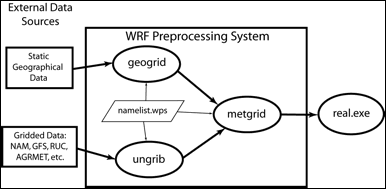
\includegraphics[width=0.65\textwidth]{image002.png}
    \caption{Construção de uma simulação \textit{real} usando o WPS. \newline Fonte: \textcite{duda2006}}.
    \label{wpsdetalha}
\end{figure}
\bigskip

\subsection{Download do WPS}
\bigskip

\noindent O WPS está incluído no pacote do COAWST, entretanto o \textit{download} do WPS, pode ser feito na página do WRF (\textcolor{bleu_cite}{\href{http://www2.mmm.ucar.edu/wrf/users/download/get\_source.html}{\textit{http://www2.mmm.ucar.edu/wrf/users/download/get\_source.html}}}). Baixe-o e adicione o arquivo \textit{tar.gz} no cluster (de preferência dentro da pasta do COAWST) com o \textit{sftp}:
\bigskip

\begin{bashcode}
sftp -P2000 nome.sobrenome@acesso-hpc.cptec.inpe.br
cd COAWST
put WPSV3.9.0.1.tar.gz
\end{bashcode}
\bigskip

\noindent Para descompactar, saia do \textit{sftp}, entre no cluster e digite:
\bigskip

\begin{bashcode}
ssh -Y nome.sobrenome@acesso-hpc.cptec.inpe.br -p 2000
cd COAWST
tar -xvzf WPSV3.9.0.1.tar.gz
\end{bashcode}
\bigskip

\subsection{Compilando o WPS no Kerana}\label{wpsker}
\bigskip

\begin{tcolorbox}[enhanced,
  grow to left by=0cm,%   equivalent to negative mdframed 'leftmargin'
  grow to right by=0cm,%  equivalent to negativ mdframed 'rightmargin'
  enlarge top by=0cm,%     equivalent to mdframed 'skipabove'
  enlarge bottom by=0cm,%  equivalent to mdframed 'skipbeow'
  tcbox raise base,
  boxrule=1.0pt,
  left=18mm,
  colframe=red!50!black,coltext=red!25!black,colback=red!10!white,
  overlay={\begin{tcbclipinterior}\fill[red!75!blue!50!white] (frame.south west)
    rectangle node[text=white,font=\sffamily\bfseries\footnotesize,rotate=0] {ATENÇÃO} ([xshift=18mm]frame.north west);\end{tcbclipinterior}}]
Como dito anteriormente, na Seção \textcolor{bleu_cite}{\ref{wpsker}}, o WPS está incluído com o COAWST. Sugere-se usar esta versão para gerar os arquivos de entrada do WRF.
\end{tcolorbox}
\bigskip

\noindent Para compilar o WPS e gerar os executáveis do programa, é necessário ativar as bibliotecas com o \textit{setup\_pgi.sh}, 
          que se encontram dentro do diretório \textit{/home/nome.sobrenome/repositorio}. Ative-os com o comando:
\bigskip

\begin{bashcode}
source setup_pgi.sh
\end{bashcode}
\bigskip

\noindent Dentro da pasta do WPS, digite o seguinte comando:
\bigskip

\begin{bashcode}
./configure
\end{bashcode}
\bigskip

\noindent Será perguntado qual a máquina e o compilador que será utilizado. Escolha a opção \textit{Cray XE/XC CLE/Linux x86\_64, PGI compiler (serial)}. Neste caso, será gerada uma mensagem que o Fortran não é compatível com o C e com o NetCDF, porém ignore.
\bigskip

\noindent Abra o arquivo \textit{configure.wps}:
\bigskip

\begin{bashcode}
nedit configure.wps
\end{bashcode}
\bigskip

\noindent Modifique:
\bigskip

\begin{bashcode}
WRF_DIR  = ../WRFV3
SFC      = ftn
SCC      = gcc
DM_CC    = cc
DM_FC    = ftn
FFLAGS   = -N255 -f free -h byteswapio
F77FLAGS = -N255 -f fixed -h byteswapio

\end{bashcode}
\bigskip

\noindent Por:
\bigskip

\begin{bashcode}
WRF_DIR  = /scratch/nome.sobrenome/WRF
SFC      = ftn
SCC      = gcc
DM_CC    = gcc
DM_FC    = ftn
FFLAGS   =
F77FLAGS =
\end{bashcode}
\bigskip

\noindent Salve as modificações e inicie a compilação com o comando:
\bigskip

\begin{bashcode}
./compile
\end{bashcode}
\bigskip

\noindent Deverá gerar os executáveis \textit{metgrid.exe} e \textit{geogrid.exe}. Porém, é possível que o \textit{ungrib.exe} não seja gerado. Neste caso, repita:
\bigskip

\begin{bashcode}
./configure
\end{bashcode}
\bigskip

\noindent Escolha a opção \textit{Linux x86\_64, PGI compiler (dmpar)}.
\bigskip

\noindent Abra novamente o \textit{configure.wps} e modifique:
\bigskip

\begin{bashcode}
WRF_DIR = ../WRFV3
SFC     = pgf90
SCC     = pgcc
DMFC    = mpif90
DMCC    = mpicc
\end{bashcode}
\bigskip

\noindent Por:
\bigskip

\begin{bashcode}
WRF_DIR = /home/nome.sobrenome/WRF
SFC     = ftn
SCC     = gcc
DMFC    = ftn
DMCC    = gcc
\end{bashcode}
\bigskip

\noindent O instalador gerará somente o \textit{ungrib.exe}

\section{Construindo o seu projeto utilizando o CFSR}
\bigskip

\noindent Uma opção de banco de dados para alimentar as simulações do modelo regional atmosférico é utilizar os dados do 
          NCEP Climate Forecast System Reanalysis (CFSR) (\textcolor{bleu_cite}{\href{http://rda.ucar.edu/datasets/ds093.0}{\textit{http://rda.ucar.edu/datasets/ds093.0}}}). 
          Esse banco de dados é uma reanálise, de janeiro de 1979 a dezembro de 2010, onde um modelo acoplado (atmosfera-oceano-superfície terrestre e gelo marinho)
          assimila dados orbitais, de cruzeiros de pesquisa, boias oceanográficas e estações meteorológicas. Esta base de dados 
          possui resolução vertical com 38 níveis, que se estendem desde a superfície até 1 hPa, com resolução temporal de 6 horas
          e horizontal de 0,5\degree para níveis de pressão e de 0,312\degree para variáveis na superfície.
\bigskip

\noindent Para acessar aos dados é necessário se cadastrar no site. Após feito isto, entre no link do banco de dados, 
          clique na guia \textit{Data Acess} e clique em \textit{Get a subset}.
\bigskip

\noindent Na próxima página, como observado na Figura \textcolor{bleu_cite}{\ref{detalhacfsr}}, escolha as datas de ínicio 
          e fim dos dados e selecione em \textit{Parameter presets} os três parâmetros do WRF (\textit{Pressure}, 
          \textit{Surface} e \textit{SST}). Só poderá ser baixado um parâmetro por vez.
\bigskip

\begin{figure}[H]
    \centering
    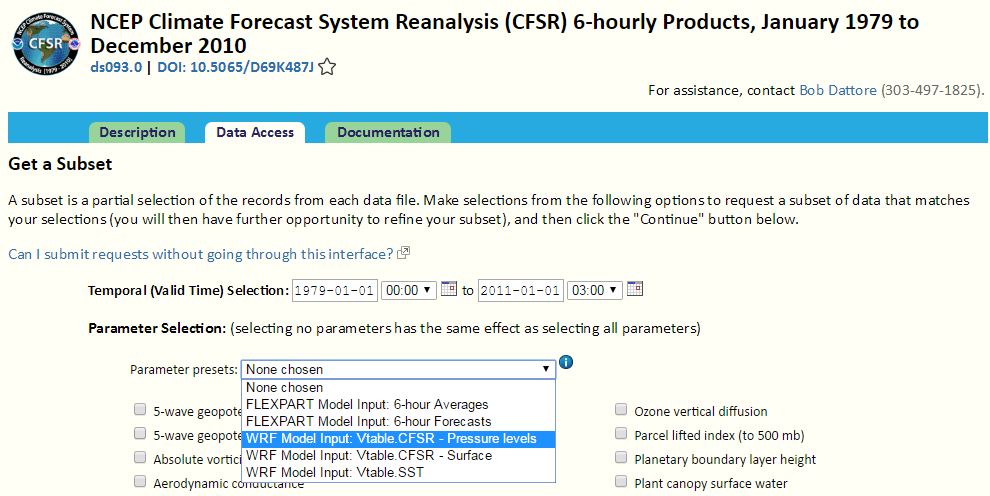
\includegraphics[width=0.95\textwidth]{1.png}
    \caption{Exemplo da página de dados do CFSR.}
    \label{detalhacfsr}
\end{figure}
\bigskip

\noindent Baixe os dados (em formato \textit{grib}) e separe-os em três pastas de acordo com os parâmetros de cada um: 
          SST, Surface e Pressure. Compacte-os e coloque no cluster:
\bigskip

\begin{bashcode}
tar -cvzf SST.tar.gz SST/
tar -cvzf Pressure.tar.gz Pressure/
tar -cvzf Surface.tar.gz Surface/
ssh -Y nome.sobrenome@acesso-hpc.cptec.inpe.br -p 2000
mkdir Dados_CFSR
exit
sftp -P2000 nome.sobrenome@acesso-hpc.cptec.inpe.br
cd Dados_CFSR
put SST.tar.gz
put Pressure.tar.gz
put Surface.tar.gz
exit
ssh -Y nome.sobrenome@acesso-hpc.cptec.inpe.br -p 2000
cd Dados_CFSR
tar -xvzf SST.tar.gz
tar -xvzf Pressure.tar.gz
tar -xvzf Surface.tar.gz
\end{bashcode}
\bigskip


\begin{tcolorbox}[enhanced,
  grow to left by=0cm,%   equivalent to negative mdframed 'leftmargin'
  grow to right by=0cm,%  equivalent to negative mdframed 'rightmargin'
  enlarge top by=0cm,%     equivalent to mdframed 'skipabove'
  enlarge bottom by=0cm,%  equivalent to mdframed 'skipbelow'
  tcbox raise base,
  boxrule=1.0pt,
  left=18mm,
  colframe=red!50!black,coltext=red!25!black,colback=red!10!white,
  overlay={\begin{tcbclipinterior}\fill[red!75!blue!50!white] (frame.south west)
    rectangle node[text=white,font=\sffamily\bfseries\footnotesize,rotate=0] {ATENÇÃO} ([xshift=18mm]frame.north west);\end{tcbclipinterior}}]
Você pode criar uma pasta de dados do CFSR na sua área. Não é preciso colocar os dados em uma pasta específica. No caso acima, os dados estão dentro da pasta Dados\_CFSR.
\end{tcolorbox}
\bigskip

\subsection{\textit{geogrid}}\label{geowps}
\bigskip

\noindent Como dito anteriormente, o \textit{geogrid} gera o domínio da grade através de dados geográficos. Os dados podem ser obtidos nesse site: (\textcolor{bleu_cite}{\href{http://www2.mmm.ucar.edu/wrf/users/download/get\_sources\_wps\_geog.html}{\textit{http://www2.mmm.ucar.edu/wrf/users/download/get\_sources\_wps\_geog.html}}}), ou então no repositório do guia a partir do diretório:
\bigskip

\begin{bashcode}
/scratch/nome.sobrenome/repositorio/COAWST/WPS/geog
\end{bashcode}
\bigskip

\noindent Com os dados do CFSR e do \textit{geogrid} em mãos, entre no diretório do WPS e abra o \textit{namelist.wps}. A estrutura do arquivo está exemplificada na Figura \textcolor{bleu_cite}{\ref{namelistwps}}:
\bigskip

\begin{bashcode}
nedit namelist.wps
\end{bashcode}
\bigskip

\begin{figure}[H]
    \centering
    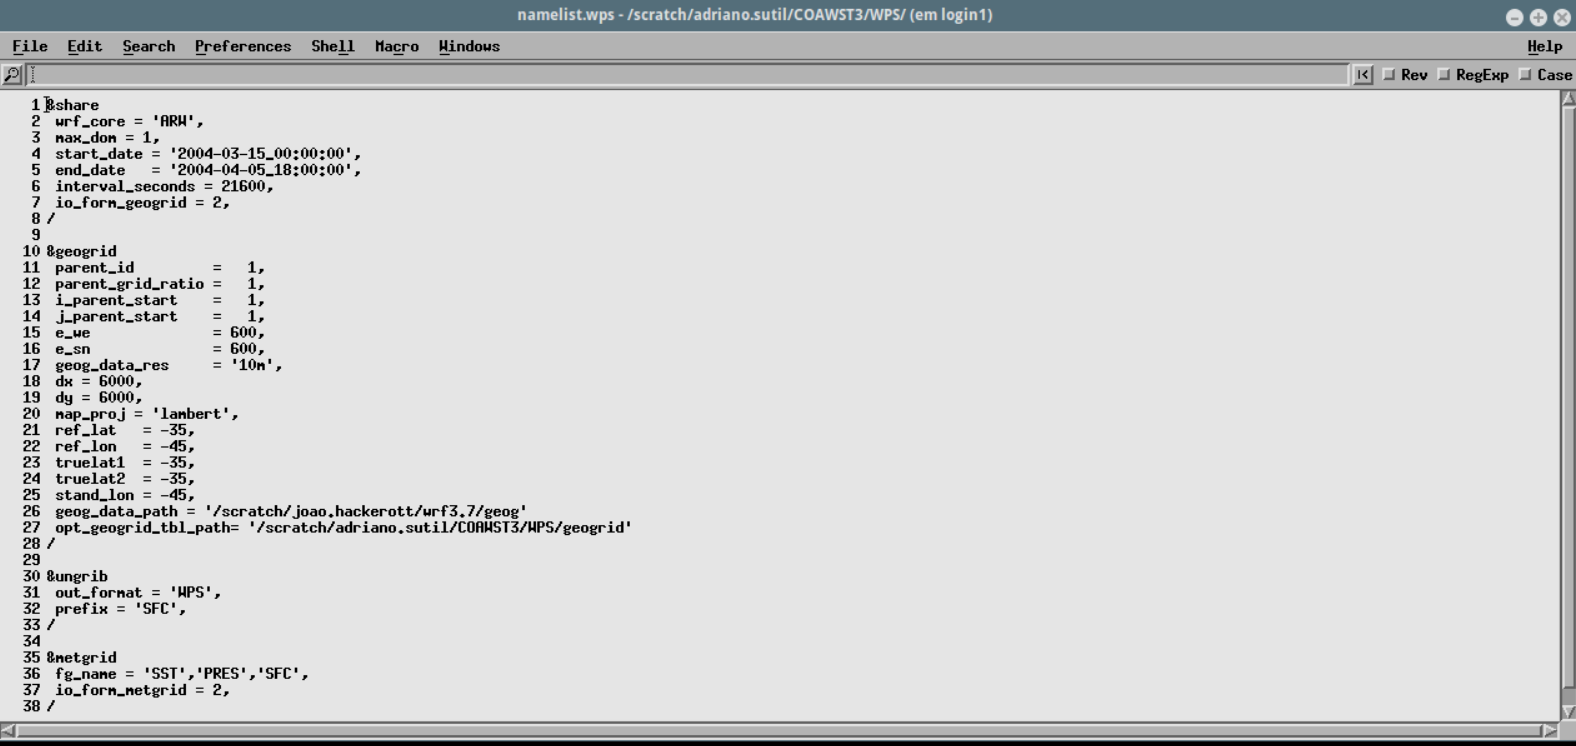
\includegraphics[width=0.95\textwidth]{image3411.png}
    \caption{Exemplo do \textit{namelist.wps}.}
    \label{namelistwps}
\end{figure}
\bigskip

\noindent Altere os diretórios \textit{geog\_data\_path}, para o diretório onde estão os dados geográficos do geog, o \textit{geog\_data\_res} caso queira utilizar outros dados geográficos e o \textit{opt\_geogrid\_tbl\_path}, que é o diretório do próprio \textit{geogrid}.
\bigskip

\noindent O WPS utiliza um marco central definido pelos pontos de latitude (\textit{ref\_lat}) e (\textit{ref\_lon}) de referência. 
          Ele gerará a grade a partir desse ponto e através da resolução espacial escolhida. 
          No caso da Figura \textcolor{bleu_cite}{\ref{namelistwps}}, será preparada uma simulação iniciando no 
          dia 15 de março de 2004 até 05 de abril de 2004, com 6 km de resolução espacial (\textit{dx} e \textit{dy} = 6000),
          em projeção lambertiana, com 600 pontos de grade. Ou seja, utilizando como referência -35\degree de latitude e -45\degree de longitude,
          será criada uma grade com 600 pontos na direção oeste-leste (\textit{e\_we}) e 600 pontos na direção sul-norte (\textit{e\_sn}), com cada 
          ponto possuindo um espaçamento de 6000 metros entre eles.
\bigskip

\noindent Para iniciar o \textit{geogrid}, é necessário o arquivo com extensão Shell (\textit{.sh}), que submete a execução do programa no Kerana. Ele se encontra no diretório \textit{/repositorio/WPS\_scripts}. Logo, mova o conteúdo da pasta para o diretório do WPS com os comandos:
\bigskip

\begin{bashcode}[fontsize=\footnotesize]
cd /home/nome.sobrenome/repositorio/WPS_scripts
mv qsub_geogrid.sh qsub_ungrib.sh qsub_metgrid.sh /home/nome.sobrenome/COAWST/WPS
\end{bashcode}
\bigskip

\noindent A estrutura do arquivo \textit{qsub\_geogrid.sh} está demonstrada na Figura \textcolor{bleu_cite}{\ref{qsubgeonedit}}. Modifique o diretório de acordo com seu usuário.
\bigskip

\begin{figure}[H]
    \centering
    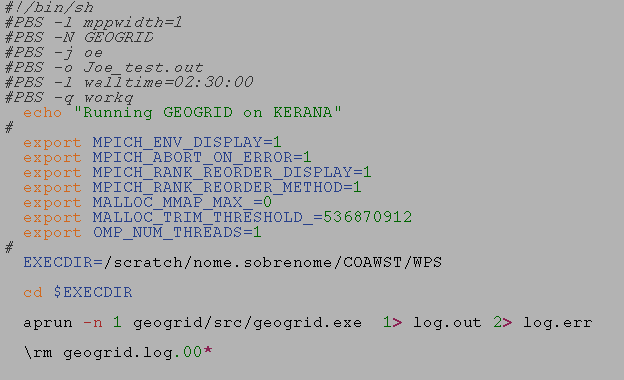
\includegraphics[width=0.95\textwidth]{qsubgeonedit.png}
    \caption{Exemplo da estrutura do arquivo \textit{qsub\_geodrid.sh}.}
    \label{qsubgeonedit}
\end{figure}
\bigskip

\noindent Para executar o \textit{geogrid}, utilize o comando \textit{qsub}:
\bigskip

\begin{bashcode}
qsub qsub_geodrid.sh
\end{bashcode}
\bigskip

\noindent Serão gerados dois arquivos para acompanhar a evolução do programa: \textit{log.err} e \textit{log.out}. Procure pela mensagem final de conclusão do programa, conforme a Figura \textcolor{bleu_cite}{\ref{qsubgeofinal}}, no arquivo \textit{log.out}.
\bigskip

\begin{figure}[H]
    \centering
    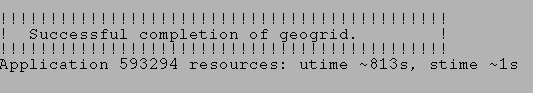
\includegraphics[width=0.55\textwidth]{qsubgeo.png}
    \caption{Exemplo de conclusão do \textit{geogrid}.}
    \label{qsubgeofinal}
\end{figure}
\bigskip

\noindent Ao concluir a execução do \textit{geogrid}, será gerado o arquivo \textit{geo\_em\_d01.nc}. É possível visualizar o arquivo NetCDF com o Ncview:
\bigskip

\begin{bashcode}
module load netcdf
ncview geo_em_d01.nc
\end{bashcode}
\bigskip

\noindent Será sempre necessário executar o \textit{geogrid} até encontrar um domínio que seja adequado para o seu projeto, pois o WPS não possui interface gráfica. Uma solução para contornar o problema é utilizar o NCAR Command Language versão 6.4 (NCL; \cite{Ncl2017}) para plotar o domínio escolhido no \textit{namelist.wps}.  Este será o tema da próxima subseção.
\bigskip

\subsection{Utilizando o NCL para plotar o domínio da grade}
\bigskip

\noindent Para instalar o NCL na sua área, mova a pasta \textit{NCL} que se encontra dentro do repositório:
\bigskip

\begin{bashcode}
mv /scratch/nome.sobrenome/repositorio/NCL /scratch/nome.sobrenome
\end{bashcode}
\bigskip

\noindent Abra o \textit{.bashrc}:
\bigskip

\begin{bashcode}
cd
nedit .bashrc
\end{bashcode}
\bigskip

\noindent Adicione as seguintes linhas de comando, alterando para o seu nome de usuário:
\bigskip

\begin{bashcode}
export NCARG_ROOT=/scratch/nome.sobrenome/NCL
export PATH=$NCARG_ROOT/bin:$PATH
\end{bashcode}
\bigskip

\noindent Salve e execute os comandos \textit{source} e de inicialização do NCL.
\bigskip

\begin{bashcode}
source .bashrc
ncl
\end{bashcode}
\bigskip

\noindent Verifique se o NCL foi inicializado como na Figura \ref{nclinit}.
\bigskip

\begin{figure}[H]
    \centering
    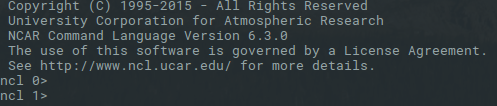
\includegraphics[width=0.95\textwidth]{nclinit.png}
    \caption{Exemplo de inicialização do NCL.}
    \label{nclinit}
\end{figure}
\bigskip


\noindent Entre no repositório e abra o arquivo \textit{plotgrids.ncl}. O código gera a imagem do domínio a partir dos dados do arquivo \textit{namelist.wps} do WPS.
\bigskip

\begin{bashcode}
cd /scratch/nome.sobrenome/repositorio
nedit plotgrids.ncl
\end{bashcode}
\bigskip

\noindent Modifique o diretório do \textit{namelist.wps} de acordo com a sua área de usuário:
\bigskip

\begin{bashcode}
filename = "/home/nome.sobrenome/COAWST/WPS/namelist.wps"
\end{bashcode}
\bigskip

\noindent Execute o código com o comando:
\bigskip

\begin{bashcode}
ncl plotgrids.ncl
\end{bashcode}
\bigskip

\noindent O código buscará os pontos de grade e a resolução do domínio através do arquivo \textit{namelist.wps} e mostrará na tela, como apresentado na Figura \textcolor{bleu_cite}{\ref{nclgrids}}. Repita o processo até encontrar um domínio adequado à sua necessidade.
\bigskip

\begin{figure}[H]
    \centering
    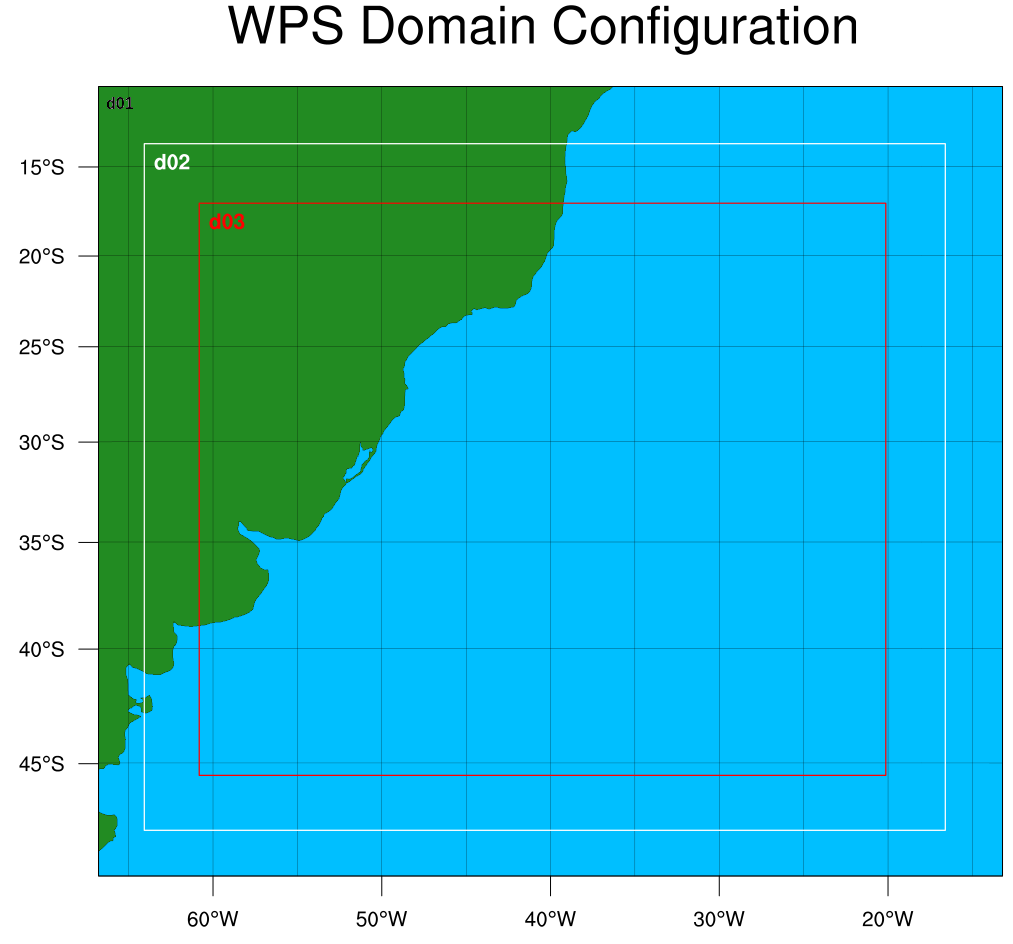
\includegraphics[width=0.65\textwidth]{wps_domain_new.png}
    \caption{Exemplo da figura gerada pelo script \textit{plotgrids.ncl}. Neste exemplo foram gerados três domínios.}
    \label{nclgrids}
\end{figure}
\bigskip


\noindent Conforme a seção \textcolor{bleu_cite}{\ref{geowps}}, para executar o \textit{geogrid}, é necessário utilizar o comando \textit{qsub}. Abra o arquivo \textit{qsub\_geogrid.sh} e mude os diretórios para o seu nome de usuário e salve. Digite o comando para executar o programa:
\bigskip

\begin{bashcode}
qsub qsub_geogrid.sh
\end{bashcode}
\bigskip

\noindent Com a execução do \textit{geogrid}, serão gerados dois arquivos para acompanhar a evolução do programa: \textit{log.err} e \textit{log.out}:
\bigskip

\begin{bashcode}
nedit log.err log.out &
\end{bashcode}
\bigskip

\noindent Ao executar o \textit{geogrid} com sucesso, uma mensagem final aparecerá no arquivo \textit{log.out}, conforme a Figura \textcolor{bleu_cite}{\ref{qsubgeofinal}}. Será gerado o arquivo \textit{geo\_em\_d01.nc}
\bigskip


\subsection{\textit{ungrib}}\label{ungribsecao}
\bigskip
\noindent Com o domínio preparado pelo \textit{geogrid}, podemos avançar para o \textit{ungrib}, que extrai os campos meteorológicos 
          e oceanográficos de arquivos com formato \textit{GRIB}. Começaremos, primeiramente, a criar os dados de SST. Abra o \textit{namelist.wps} 
          e na seção \textit{\&ungrib}, altere o \textit{prefix} para \textit{SST}, conforme a Figura \ref{ungribprefix} e salve.
\bigskip

\begin{figure}[H]
    \centering
    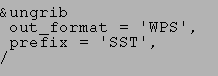
\includegraphics[width=0.45\textwidth]{ungribprefix.png}
    \caption{Exemplo da seção \textit{\&ungrib} do \textit{namelist.wps}.}
    \label{ungribprefix}
\end{figure}
\bigskip

\noindent Importe a \textit{Variable Table} de SST do WPS através de um link simbólico. Digite no terminal:
\bigskip

\begin{bashcode}
ln -sf ungrib/Variable_Tables/Vtable.SST Vtable
\end{bashcode}
\bigskip

\begin{tcolorbox}[enhanced,
  grow to left by=0cm,%   equivalent to negative mdframed 'leftmargin'
  grow to right by=0cm,%  equivalent to negative mdframed 'rightmargin'
  enlarge top by=0cm,%     equivalent to mdframed 'skipabove'
  enlarge bottom by=0cm,%  equivalent to mdframed 'skipbelow'
  tcbox raise base,
  boxrule=1.0pt,
  left=18mm,
  colframe=red!50!black,coltext=red!25!black,colback=red!10!white,
  overlay={\begin{tcbclipinterior}\fill[red!75!blue!50!white] (frame.south west)
    rectangle node[text=white,font=\sffamily\bfseries\footnotesize,rotate=0] {ATENÇÃO} ([xshift=18mm]frame.north west);\end{tcbclipinterior}}]
A \textit{Vtable} é utilizada para ler os arquivos em formato \textit{grib}. É importante utilizar a \textit{Vtable} correspondente para o banco de dados escolhido. Você pode consultá-las em \textit{WPS/ungrib/Variable\_Tables}
\end{tcolorbox}
\bigskip

\noindent Crie diversos links simbólicos com os dados de SST do CFSR através do arquivo \textit{link\_grib.csh} apontando o diretório dos dados:
\bigskip

\begin{bashcode}
./link_grib.csh /scratch/nome.sobrenome/Dados_CFSR/SST/*
\end{bashcode}
\bigskip

\noindent Abra o arquivo \textit{qsub\_ungrib.sh} e modifique o diretório de acordo com o seu usuário e  digite:
\bigskip

\begin{bashcode}
qsub qsub_ungrib.sh
\end{bashcode}
\bigskip

\begin{tcolorbox}[enhanced,
  grow to left by=0cm,%   equivalent to negative mdframed 'leftmargin'
  grow to right by=0cm,%  equivalent to negative mdframed 'rightmargin'
  enlarge top by=0cm,%     equivalent to mdframed 'skipabove'
  enlarge bottom by=0cm,%  equivalent to mdframed 'skipbelow'
  tcbox raise base,
  boxrule=1.0pt,
  left=18mm,
  colframe=red!50!black,coltext=red!25!black,colback=red!10!white,
  overlay={\begin{tcbclipinterior}\fill[red!75!blue!50!white] (frame.south west)
    rectangle node[text=white,font=\sffamily\bfseries\footnotesize,rotate=0] {ATENÇÃO} ([xshift=18mm]frame.north west);\end{tcbclipinterior}}]
O arquivo \textit{qsub\_ungrib.sh} se encontra dentro da pasta \textit{/repositorio/WPS\_scripts}.
\end{tcolorbox}
\bigskip

\noindent Serão criados diversos arquivos com inicial \textit{SST:} seguido da data escolhida para a integração. Para checar o sucesso ao executar o ungrib, procure pela mensagem da Figura \textcolor{bleu_cite}{\ref{ungribsucess}} ao final do arquivo \textit{log.out}.
\bigskip

\begin{figure}[H]
    \centering
    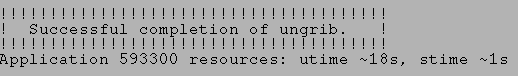
\includegraphics[width=0.45\textwidth]{qsubung.png}
    \caption{Mensagem final no arquivo \textit{log.out} ao executar o \textit{ungrib}.}
    \label{ungribsucess}
\end{figure}
\bigskip

\noindent Seguiremos para os dados de superfície do CFSR. Altere o \textit{prefix} no \textit{namelist.wps} (Figura \textcolor{bleu_cite}{\ref{ungribprefix}}). Modifique \textit{SST} por \textit{SFC} e salve a modificação.
\bigskip

\noindent Importe a \textit{Variable Table} do CFSR no WPS com o comando de criação de link simbólico:
\bigskip

\begin{bashcode}
ln -sf ungrib/Variable_Tables/Vtable.CFSR Vtable
\end{bashcode}
\bigskip

\noindent Crie os links simbólicos dos dados de superfície do CFSR com o comando abaixo e execute o \textit{ungrib} mais uma vez:
\bigskip

\begin{bashcode}
./link_grib.csh /scratch/nome.sobrenome/Dados_CFSR/Surface/*
qsub qsub_ungrib.sh
\end{bashcode}
\bigskip

\noindent Procure pela mensagem final conforme identificada na Figura \textcolor{bleu_cite}{\ref{ungribsucess}}.
\bigskip

\noindent Altere o \textit{prefix} do \textit{namelist.wps} (Figura \textcolor{bleu_cite}{\ref{ungribprefix}}), substitua \textit{SFC} por \textit{PRES} e salve o arquivo.
\bigskip

\noindent Crie os links simbólicos para os dados de pressão e execute o \textit{ungrib}:
\bigskip

\begin{bashcode}
./link_grib.csh /scratch/nome.sobrenome/Dados_CFSR/Pressure/*
qsub qsub_ungrib.sh
\end{bashcode}
\bigskip

\noindent Por fim, procure pela mensagem final conforme identificada na Figura \textcolor{bleu_cite}{\ref{ungribsucess}}. Ao finalizar estes passos, constarão diversos arquivos com as iniciais \textit{SST}, \textit{PRES}, \textit{SFC} seguidos com as datas do período de integração escolhidas.
\bigskip




\subsection{\textit{metgrid}}\label{metgridsecao}
\bigskip
\noindent Para interpolar os dados gerados pelo \textit{ungrib.exe},  abra o \textit{namelist.wps} e altere na guia \textit{fg\_name} os nomes utilizados no \textit{ungrib}. No caso anterior, foram utilizados \textit{PRES}, \textit{SFC} e \textit{SST}, como no exemplo da Figura \textcolor{bleu_cite}{\ref{fgname}}:
\bigskip

\begin{figure}[H]
    \centering
    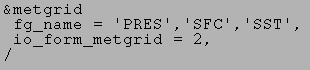
\includegraphics[width=0.5\textwidth]{fgname.png}
    \caption{Exemplo da guia do \textit{metgrid} no \textit{namelist.wps}.}
    \label{fgname}
\end{figure}
\bigskip

\noindent Abra e mude o diretório do arquivo \textit{qsub\_metgrid.sh} e execute:
\bigskip

\begin{bashcode}
qsub qsub_metgrid.sh
\end{bashcode}
\bigskip

\noindent Mova os arquivos gerados pelo \textit{metgrid} (\textit{met\_em.d01*}) para o diretório dos casos reais do WRF:
\bigskip

\begin{bashcode}
 mv met_em.d01* /home/nome.sobrenome/WRF/test/em_real
\end{bashcode}
\bigskip

\subsection{\textit{real}}\label{realsecao}
\bigskip

\noindent Usaremos o programa \textit{real.exe} para gerar os arquivos para serem utilizados no WRF. Abra o arquivo \textit{namelist.input}, que se encontra na pasta do WRF (\textit{/home/nome.sobrenome/WRF/test/em\_real}) e modifique de acordo com o seu domínio e tempo de simulação escolhidos no \textit{namelist.wps}.
\bigskip

\noindent Para que o WRF faça a integração da TSM, é necessário incluir as seguintes variáveis ao final da seção \textit{\&time\_control} (Figura \textcolor{bleu_cite}{\ref{timecontrolnamelist}}):
\bigskip

\begin{bashcode}
io_form_auxinput4  = 2,
auxinput4_inname   = "wrflowinp_d<domain>",
auxinput4_interval = 360,
\end{bashcode}
\bigskip

\noindent O \textit{io\_form\_auxinput4} se refere ao formato final do arquivo \textit{wrflowinp} que será gerado pelo \textit{real}, o \textit{auxinput4\_inname} é o nome do arquivo de condição de fronteira para a TSM e o \textit{auxinput4\_interval} é o intervalo de tempo, em minutos, do arquivo de fronteira.
\bigskip

\begin{figure}[H]
    \centering
    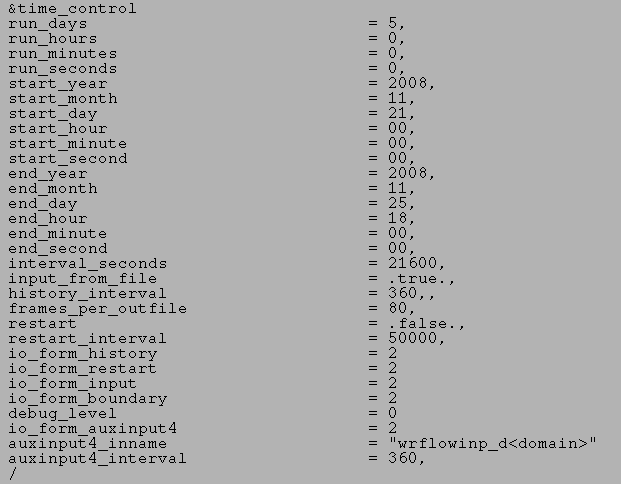
\includegraphics[width=0.70\textwidth]{namelisttimecontrol.png}
    \caption{Exemplo da guia \textit{\&time\_control} no \textit{namelist.input}.}
    \label{timecontrolnamelist}
\end{figure}
\bigskip

\noindent Inclua também, na seção \textit{\&physics} (Figura \textcolor{bleu_cite}{\ref{physicsnamelist}}) no \textit{namelist.input} a opção para atualizar a TSM:
\bigskip

\begin{bashcode}
sst_update = 1,
\end{bashcode}
\bigskip

\begin{figure}[H]
    \centering
    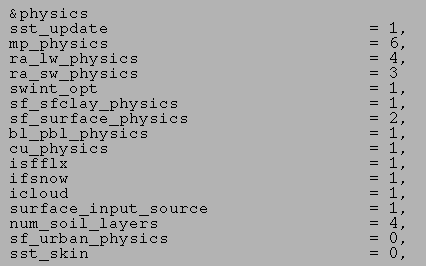
\includegraphics[width=0.70\textwidth]{physics.png}
    \caption{Exemplo da guia \textit{\&physics} no \textit{namelist.input} com \textit{sst\_update} = 1 para atualizar a TSM ao longo do tempo.}
    \label{physicsnamelist}
\end{figure}
\bigskip

\noindent Após concluir as modificações, é preciso utilizar o arquivo \textit{qsub\_real.sh} para submeter a operação. O arquivo está localizado no diretório \textit{/repositorio/WRF\_scripts}. Mova o arquivo para a pasta \textit{em\_real} do WRF, mude o diretório de acordo com o seu usuário e execute:
\bigskip

\begin{bashcode}
cd /home/nome.sobrenome/repositorio/WRF_scripts
mv qsub_real.sh /home/nome.sobrenome/WRF/test/em_real
qsub qsub_real.sh
\end{bashcode}
\bigskip

\begin{tcolorbox}[enhanced,
  grow to left by=0cm,%   equivalent to negative mdframed 'leftmargin'
  grow to right by=0cm,%  equivalent to negative mdframed 'rightmargin'
  enlarge top by=0cm,%     equivalent to mdframed 'skipabove'
  enlarge bottom by=0cm,%  equivalent to mdframed 'skipbelow'
  tcbox raise base,
  boxrule=1.0pt,
  left=18mm,
  colframe=red!50!black,coltext=red!25!black,colback=red!10!white,
  overlay={\begin{tcbclipinterior}\fill[red!75!blue!50!white] (frame.south west)
    rectangle node[text=white,font=\sffamily\bfseries\footnotesize,rotate=0] {ATENÇÃO} ([xshift=18mm]frame.north west);\end{tcbclipinterior}}]
O arquivo \textit{qsub\_real.sh} se encontra dentro da pasta \textit{/repositorio/WRF\_scripts}.
\end{tcolorbox}
\bigskip

\noindent Para atestar o sucesso em executar o \textit{real}, procure no final do arquivo \textit{log.out} pela mensagem de sucesso conforme exemplificada na Figura \textcolor{bleu_cite}{\ref{realfinish}}.
\bigskip

\begin{figure}[H]
    \centering
    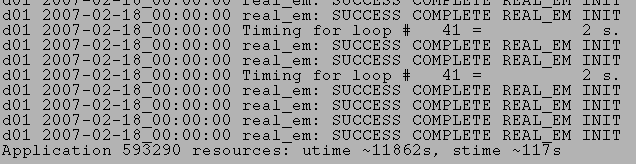
\includegraphics[width=0.70\textwidth]{realsucess.png}
    \caption{Exemplo da finalização com sucesso do \textit{real}.}
    \label{realfinish}
\end{figure}
\bigskip


\noindent Ao completar o \textit{real}, serão gerados três arquivos: \textit{wrfbdy\_d01}, \textit{wrfinput\_d01} e \textit{wrflowinp\_d01} caso tenha escolhido somente um domínio, isto é, sem aninhamento. Após isso, as condições do WRF estão prontas para serem copiadas para a sua pasta de projetos no COAWST:
\bigskip

\begin{bashcode}[fontsize=\scriptsize]
cp wrfbdy_d01 wrfinput_d01 wrflowinp_d01 /home/nome.sobrenome/COAWST/Projects/nome_do_projeto
\end{bashcode}
\bigskip

\section{Usando o WRF}\label{wrfsecao2}
\bigskip

\noindent Com as condições do WRF prontas, é possível iniciar a simulação do seu projeto utilizando somente o WRF.
\bigskip

\noindent Para executar a simulação no cluster, é necessário utilizar o arquivo \textit{qsub\_wrf.sh}. Ele está localizado no diretório \textit{/repositorio/WRF\_scripts}. Mova o arquivo para a pasta \textit{em\_real} do WRF, modique o diretório de acordo com o seu usuário e salve:
\bigskip

\begin{bashcode}
cd /home/nome.sobrenome/repositorio/WRF_scripts
mv qsub_wrf.sh /home/nome.sobrenome/WRF/test/em_real
nedit qsub_wrf.sh
\end{bashcode}
\bigskip

\noindent Para iniciar a simulação, execute:
\bigskip

\begin{bashcode}
qsub qsub_wrf.sh
\end{bashcode}
\bigskip

\begin{tcolorbox}[enhanced,
  grow to left by=0cm,%   equivalent to negative mdframed 'leftmargin'
  grow to right by=0cm,%  equivalent to negative mdframed 'rightmargin'
  enlarge top by=0cm,%     equivalent to mdframed 'skipabove'
  enlarge bottom by=0cm,%  equivalent to mdframed 'skipbelow'
  tcbox raise base,
  boxrule=1.0pt,
  left=18mm,
  colframe=red!50!black,coltext=red!25!black,colback=red!10!white,
  overlay={\begin{tcbclipinterior}\fill[red!75!blue!50!white] (frame.south west)
    rectangle node[text=white,font=\sffamily\bfseries\footnotesize,rotate=0] {ATENÇÃO} ([xshift=18mm]frame.north west);\end{tcbclipinterior}}]
O arquivo \textit{qsub\_wrf.sh} se encontra dentro da pasta \textit{/repositorio/WRF\_scripts}.
\end{tcolorbox}
\bigskip

\noindent Acompanhe a evolução da simulação a partir dos arquivos \textit{log.out} e \textit{log.err}. Caso opte pela informação ser atualizada pelo terminal, digite:
\bigskip

\begin{bashcode}
tail -f log.out
\end{bashcode}
\bigskip
